\documentclass[a4paper,12pt]{article}
\usepackage{graphicx} 
\usepackage{hyperref}
\usepackage{float}

% \begin{figure}[H]
%     \centering
%     \includegraphics[width=0.7\textwidth]{filename.png}
%     \caption{Your figure caption here.}
%     \label{fig:yourlabel}
% \end{figure}

\begin{document}

\title{Data Science - Assignment 2 \\
Ride Sharing Analysis - Uber \& Lyft}
\author{Mohammad Hossein Basouli}
\date{\today}
\maketitle

\section*{Linear \& Polynomial Models}

\subsection*{Data Preprocessing}

\textbf{Data Reduction}: We remove irrelavant features as well as redundant features. e.g. 'id', 'timestamp', 'timezone', 'datetime', 'visibility.1',
'temperatureMinTime', 'temperatureMax', 'temperatureMaxTime',
'apparentTemperatureMin', 'apparentTemperatureMinTime',
'apparentTemperatureMax', 'apparentTemperatureMaxTime' \\ 

\noindent\textbf{Data Transformation}: 
\begin{itemize}
    \item extraction of \textbf{sunriseHour} and \textbf{sunsetHour}.
    \item encoding of categorical features via \textbf{One-Hot Encoding}.
\end{itemize}

\subsection*{Exploratory Data Analysis}

\textbf{High Correlated Features}: Features with a correlation absolute value greater than 0.05: \\ 
\begin{table}[H]
    \centering
    \begin{tabular}{|l|r|}
    \hline
    \textbf{Feature} & \textbf{Value} \\
    \hline
    price & 1.000000 \\
    distance & 0.333871 \\
    surge\_multiplier & 0.165611 \\
    source\_Boston University & 0.067880 \\
    source\_Fenway & 0.057167 \\
    source\_Haymarket Square & -0.101514 \\
    destination\_Boston University & 0.072743 \\
    destination\_Fenway & 0.053153 \\
    destination\_Haymarket Square & -0.075808 \\
    destination\_South Station & -0.055659 \\
    cab\_type\_Uber & -0.068606 \\
    product\_id\_6c84fd89-3f11-4782-9b50-97c468b19529 & 0.195100 \\
    product\_id\_6d318bcc-22a3-4af6-bddd-b409bfce1546 & 0.412593 \\
    product\_id\_997acbb5-e102-41e1-b155-9df7de0a73f2 & -0.300286 \\
    product\_id\_9a0e7b09-b92b-4c41-9779-2ad22b4d779d & -0.236477 \\
    product\_id\_lyft & -0.239700 \\
    product\_id\_lyft\_line & -0.426482 \\
    product\_id\_lyft\_lux & 0.245791 \\
    product\_id\_lyft\_luxsuv & 0.412894 \\
    product\_id\_lyft\_premier & 0.107153 \\
    name\_Black SUV & 0.412593 \\
    name\_Lux & 0.107153 \\
    name\_Lux Black & 0.245791 \\
    name\_Lux Black XL & 0.412894 \\
    name\_Lyft & -0.239700 \\
    name\_Shared & -0.426482 \\
    name\_UberPool & -0.300286 \\
    name\_UberX & -0.236468 \\
    name\_WAV & -0.236477 \\
    \hline
    \end{tabular}
    \caption{Features with a correlation absolute value greater than 0.05}
    \label{tab:tab_1}
\end{table}    
\noindent\textbf{Feature Selection}: At the begining I have utilized \textbf{sklearn univariate feature selection} methods such as \textbf{VarianceThreshold}, \textbf{SelectKBest} and \textbf{SelectPercentile} along with metrics such as \textbf{r\_regression}, \textbf{f\_regression} and \textbf{mutual\_info\_regression}, but they all gave poor results. It might be due to this fact that these methods might not work in some cases, e.g. for a dataset which even the low correlated features lead to a significant, important information in our analysis. This might be the case, since we haven't got good results .Thus, we approach the \textbf{Feature Selection} process by another method, like examining the relation of correlated features with the target variable by hand. It turns out that this approach leads to very decent results, thus, we will only maintain features that are listed in the table~\ref{tab:tab_1}. 

\noindent\textbf{Outliers}: First, we have removed the outliers from our dataset but it did no good. Also the dataset size is very large, even if the dataset contains outliers, this could be ignored because our sample size is enough in order to make the model robus to the outliers. Thus we keep all of the rows.

\subsection*{Train-Test Splitting}
20\% Test, 80\% Train

\subsection*{Linear Models}

\subsubsection*{Base Linear Regression With Missing \textbf{price} Dropped}

\textbf{Evaluation}: 
\begin{table}[H]
    \centering
    \begin{tabular}{|l|c|c|}
    \hline
    \textbf{Metric} & \textbf{Train} & \textbf{Test} \\
    \hline
    MSE & 6.2973 & 6.3036 \\
    MAE & 1.7688 & 1.7684 \\
    $R^2$ & 0.9275 & 0.9277 \\
    \hline
    \end{tabular}
    \caption{Evaluation of Base Linear Regression With Missing \textbf{price} Dropped}
    \label{tab:tab_2}
\end{table}

\noindent\textbf{Coefficients}: 
\begin{table}[H]
    \centering
    \begin{tabular}{|l|r|}
    \hline
    \textbf{Feature} & \textbf{Coefficient} \\
    \hline
    distance & 3.248531 \\
    product\_id\_lyft\_luxsuv & 2.314652 \\
    name\_Lux Black XL & 2.314652 \\
    name\_Black SUV & 2.051601 \\
    product\_id\_6d318bcc-22a3-4af6-bddd-b409bfce1546 & 2.051601 \\
    surge\_multiplier & 1.750053 \\
    name\_UberX & -1.659294 \\
    product\_id\_6c84fd89-3f11-4782-9b50-97c468b19529 & 1.358077 \\
    name\_Shared & -1.165846 \\
    product\_id\_lyft\_line & -1.165846 \\
    product\_id\_lyft\_lux & 1.053897 \\
    name\_Lux Black & 1.053897 \\
    name\_UberPool & -0.973288 \\
    product\_id\_997acbb5-e102-41e1-b155-9df7de0a73f2 & -0.973288 \\
    product\_id\_9a0e7b09-b92b-4c41-9779-2ad22b4d779d & -0.829638 \\
    name\_WAV & -0.829638 \\
    name\_Lyft & -0.776932 \\
    product\_id\_lyft & -0.776932 \\
    cab\_type\_Uber & 0.528733 \\
    product\_id\_lyft\_premier & 0.336811 \\
    \hline
    \end{tabular}
    \caption{Top features with corresponding coefficients}
    \label{tab:tab_3}
\end{table}

\noindent\textbf{Residual Plot}: 
\begin{figure}[H]
    \centering
    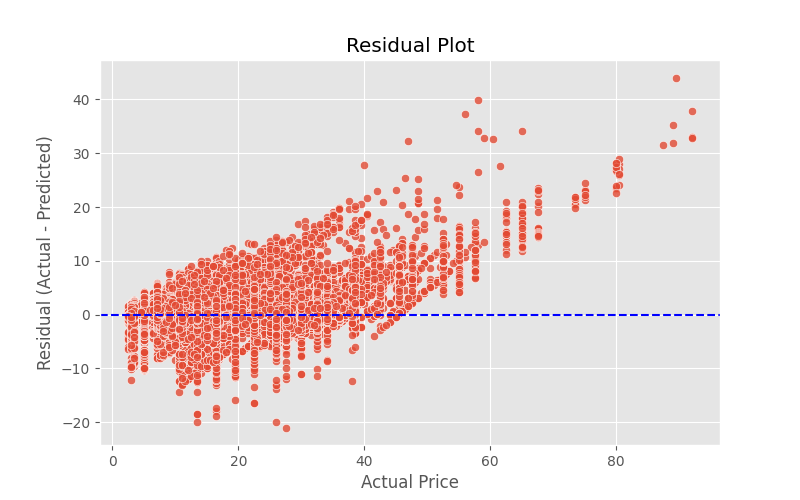
\includegraphics[width=0.7\textwidth]{./images/residual_of_base_lr.png}
    \caption{Residual Plot of Base Linear Regression With Missing \textbf{price} dropped.}
    \label{fig:fig_1}
\end{figure}

\subsubsection*{Base Linear Regression With Missing \textbf{price} Returned Back to The Training Set}

\textbf{Evaluation}: 
\begin{table}[H]
    \centering
    \begin{tabular}{|l|c|c|}
    \hline
    \textbf{Metric} & \textbf{Train} & \textbf{Test} \\
    \hline
    MSE & 32.8414 & 32.8825 \\
    MAE & 3.1355 & 3.1392 \\
    $R^2$ & 0.6220 & 0.6228 \\
    \hline
    \end{tabular}
    \caption{Evaluation of Base Linear Regression With Missing \textbf{price} Returned Back to The Training Set}
    \label{tab:tab_4}
\end{table}
    
% \textbf{Coefficients}: \\ 
% \textbf{Residual Plot}: \\ 

\subsubsection*{Regularized Linear Ridge Regression}

\textbf{Evaluation}: 
\begin{table}[H]
    \centering
    \begin{tabular}{|l|c|c|}
    \hline
    \textbf{Metric} & \textbf{Train} & \textbf{Test} \\
    \hline
    MSE & 6.2973 & 6.3036 \\
    MAE & 1.7688 & 1.7684 \\
    $R^2$ & 0.9275 & 0.9277 \\
    \hline
    \end{tabular}
    \caption{Evaluation of Regularized Linear Ridge Regression}
    \label{tab:tab_5}
\end{table}    
% \textbf{Coefficients}: \\ 
% \textbf{Residual Plot}: \\ 

\subsubsection*{Regularized Linear Lasso Regression}

\textbf{Evaluation}: 
\begin{table}[H]
    \centering
    \begin{tabular}{|l|c|c|}
    \hline
    \textbf{Metric} & \textbf{Train} & \textbf{Test} \\
    \hline
    MSE & 6.2973 & 6.3037 \\
    MAE & 1.7683 & 1.7679 \\
    $R^2$ & 0.9275 & 0.9277 \\
    \hline
    \end{tabular}
    \caption{Evaluation of Regularized Linear Lasso Regression}
    \label{tab:tab_6}
\end{table}    
% \textbf{Coefficients}: \\ 
% \textbf{Residual Plot}: \\ 

\subsection*{Polynomial Models}

\subsubsection*{Quadratic Model With Ridge Regression}

\textbf{Best Alpha}: 10

\noindent\textbf{Evaluation}: 
\begin{table}[H]
    \centering
    \begin{tabular}{|l|c|c|}
    \hline
    \textbf{Metric} & \textbf{Train} & \textbf{Test} \\
    \hline
    MSE & 3.4229 & 3.3842 \\
    MAE & 1.2621 & 1.2582 \\
    $R^2$ & 0.9606 & 0.9612 \\
    \hline
    \end{tabular}
    \caption{Evaluation of Quadratic Model With Ridge Regression}
    \label{tab:tab_7}
\end{table}
% \textbf{Coefficients}: \\ 
% \textbf{Residual Plot}: \\ 

\subsubsection*{Quadratic Model With Lasso Regression}

\textbf{Best Alpha}: 0.001

\noindent\textbf{Evaluation}: 
\begin{table}[H]
    \centering
    \begin{tabular}{|l|c|c|}
    \hline
    \textbf{Metric} & \textbf{Train} & \textbf{Test} \\
    \hline
    MSE & 3.4232 & 3.3843 \\
    MAE & 1.2621 & 1.2582 \\
    $R^2$ & 0.9606 & 0.9612 \\
    \hline
    \end{tabular}
    \caption{Evaluation of Quadratic Model With Lasso Regression}
    \label{tab:tab_8}
\end{table}
% \textbf{Coefficients}: \\ 
% \textbf{Residual Plot}: \\ 

\section*{Enhanced Model}

\subsection*{Data Preprocessing}

\textbf{Data Reduction}: We remove irrelavant \& redundant features. e.g. 'id', 'timestamp', 'timezone', 'datetime', 'visibility.1',
'temperatureMinTime', 'temperatureMax', 'temperatureMaxTime',
'apparentTemperatureMin', 'apparentTemperatureMinTime',
'apparentTemperatureMax', 'apparentTemperatureMaxTime' \\

\noindent\textbf{Data Transformation}: 
\begin{itemize}
    \item encoding of nominal categorical features via \textbf{One-Hot Encoding}
    \item encoding of ordinal categorical features via \textbf{Label Encoding}. This could improve our results since maintains difference in order of the labels in the column.
    \item extract \textbf{sunriseHour} and \textbf{sunsetHour}
\end{itemize}

\noindent\textbf{Missing Values}: We will drop the rows which have missing value on \textbf{price}.

\subsection*{Train-Test Splitting}
20\% Test, 80\% Train

\subsection*{Evaluation}
\begin{table}[H]
    \centering
    \begin{tabular}{|l|c|c|}
    \hline
    \textbf{Metric} & \textbf{Train} & \textbf{Test} \\
    \hline
    MSE & 3.0890 & 3.0483 \\
    MAE & 1.1793 & 1.1751 \\
    $R^2$ & 0.9644 & 0.9650 \\
    \hline
    \end{tabular}
    \caption{Model performance metrics on training and test sets}
    \label{tab:model-metrics}
\end{table}


% \subsection*{Coefficients}

\subsection*{Residual Plot}

\begin{figure}[H]
    \centering
    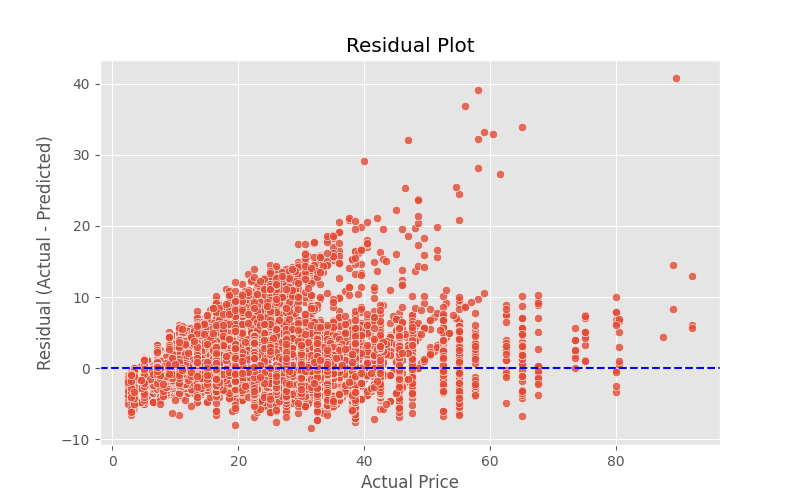
\includegraphics[width=0.7\textwidth]{./images/residual_of_enhanced.png}
    \caption{Residual Plot of Enhanced Model}
    \label{fig:fig_2}
\end{figure}


\section*{Conclusion}

\textbf{Best Model}: The best model is \textbf{Enhanced Model} which has the lowest \textbf{MSE}, \textbf{MAE} and also has the highest $R^2$ score which means the model explain much of the variance that exists whithin the data (both in \textbf{Train} and \textbf{Test} evaluation). This could be due to better encoding of ordinal features, e.g. \textbf{name} feature, as well as using good regularization regressions such as \textbf{Ridge Regression} which helps to avoid overfitting.


\end{document}